% Options for packages loaded elsewhere
\PassOptionsToPackage{unicode}{hyperref}
\PassOptionsToPackage{hyphens}{url}
%
\documentclass[
  ignorenonframetext,
]{beamer}
\usepackage{pgfpages}
\setbeamertemplate{caption}[numbered]
\setbeamertemplate{caption label separator}{: }
\setbeamercolor{caption name}{fg=normal text.fg}
\beamertemplatenavigationsymbolsempty
% Prevent slide breaks in the middle of a paragraph
\widowpenalties 1 10000
\raggedbottom
\setbeamertemplate{part page}{
  \centering
  \begin{beamercolorbox}[sep=16pt,center]{part title}
    \usebeamerfont{part title}\insertpart\par
  \end{beamercolorbox}
}
\setbeamertemplate{section page}{
  \centering
  \begin{beamercolorbox}[sep=12pt,center]{part title}
    \usebeamerfont{section title}\insertsection\par
  \end{beamercolorbox}
}
\setbeamertemplate{subsection page}{
  \centering
  \begin{beamercolorbox}[sep=8pt,center]{part title}
    \usebeamerfont{subsection title}\insertsubsection\par
  \end{beamercolorbox}
}
\AtBeginPart{
  \frame{\partpage}
}
\AtBeginSection{
  \ifbibliography
  \else
    \frame{\sectionpage}
  \fi
}
\AtBeginSubsection{
  \frame{\subsectionpage}
}
\usepackage{amsmath,amssymb}
\usepackage{lmodern}
\usepackage{iftex}
\ifPDFTeX
  \usepackage[T1]{fontenc}
  \usepackage[utf8]{inputenc}
  \usepackage{textcomp} % provide euro and other symbols
\else % if luatex or xetex
  \usepackage{unicode-math}
  \defaultfontfeatures{Scale=MatchLowercase}
  \defaultfontfeatures[\rmfamily]{Ligatures=TeX,Scale=1}
\fi
% Use upquote if available, for straight quotes in verbatim environments
\IfFileExists{upquote.sty}{\usepackage{upquote}}{}
\IfFileExists{microtype.sty}{% use microtype if available
  \usepackage[]{microtype}
  \UseMicrotypeSet[protrusion]{basicmath} % disable protrusion for tt fonts
}{}
\makeatletter
\@ifundefined{KOMAClassName}{% if non-KOMA class
  \IfFileExists{parskip.sty}{%
    \usepackage{parskip}
  }{% else
    \setlength{\parindent}{0pt}
    \setlength{\parskip}{6pt plus 2pt minus 1pt}}
}{% if KOMA class
  \KOMAoptions{parskip=half}}
\makeatother
\usepackage{xcolor}
\newif\ifbibliography
\usepackage{graphicx}
\makeatletter
\def\maxwidth{\ifdim\Gin@nat@width>\linewidth\linewidth\else\Gin@nat@width\fi}
\def\maxheight{\ifdim\Gin@nat@height>\textheight\textheight\else\Gin@nat@height\fi}
\makeatother
% Scale images if necessary, so that they will not overflow the page
% margins by default, and it is still possible to overwrite the defaults
% using explicit options in \includegraphics[width, height, ...]{}
\setkeys{Gin}{width=\maxwidth,height=\maxheight,keepaspectratio}
% Set default figure placement to htbp
\makeatletter
\def\fps@figure{htbp}
\makeatother
\setlength{\emergencystretch}{3em} % prevent overfull lines
\providecommand{\tightlist}{%
  \setlength{\itemsep}{0pt}\setlength{\parskip}{0pt}}
\setcounter{secnumdepth}{-\maxdimen} % remove section numbering
\ifLuaTeX
  \usepackage{selnolig}  % disable illegal ligatures
\fi
\IfFileExists{bookmark.sty}{\usepackage{bookmark}}{\usepackage{hyperref}}
\IfFileExists{xurl.sty}{\usepackage{xurl}}{} % add URL line breaks if available
\urlstyle{same} % disable monospaced font for URLs
\hypersetup{
  hidelinks,
  pdfcreator={LaTeX via pandoc}}

\author{}
\date{\vspace{-2.5em}}

\begin{document}

\begin{frame}{AEB 3103 Principles of Food and Resource Economics}
\protect\hypertarget{aeb-3103-principles-of-food-and-resource-economics}{}
\begin{block}{Module 6: The Economics of Taxation}
\protect\hypertarget{module-6-the-economics-of-taxation}{}
\end{block}
\end{frame}

\begin{frame}{}
\protect\hypertarget{section}{}
\emph{In this world nothing can be said to be certain, except death and
taxes} - Benjamin Franklin
\end{frame}

\begin{frame}{}
\protect\hypertarget{section-1}{}
What is the first word you think about when you think about tax?
\end{frame}

\begin{frame}{Type of taxes}
\protect\hypertarget{type-of-taxes}{}
\begin{itemize}
\tightlist
\item
  Exercise tax: tax on goods and services

  \begin{itemize}
  \tightlist
  \item
    Everything you buy, you pay 6\% tax in Florida
  \item
    OR and NH has no exercise tax
  \end{itemize}
\item
  Income tax: tax on income

  \begin{itemize}
  \tightlist
  \item
    Different brackets; federal and state income taxes
  \end{itemize}
\item
  Corporate tax
\item
  Capital gain tax
\item
  Tariff
\end{itemize}
\end{frame}

\begin{frame}{And here's a couple of statement about taxes. Are they
correct?}
\protect\hypertarget{and-heres-a-couple-of-statement-about-taxes.-are-they-correct}{}
\begin{itemize}
\tightlist
\item
  Tax only affects those who actually pay taxes.

  \begin{itemize}
  \tightlist
  \item
    For example, taxing Canadian steel = Canada will pay for that tax.
  \item
    Taxing food and beverage = consumers will pay for that tax
  \end{itemize}
\item
  Lower taxes stimulates consumption, which boosts the economy through
  multiplier effects.
\item
  Income tax makes people less likely to work.
\end{itemize}
\end{frame}

\begin{frame}{}
\protect\hypertarget{section-2}{}
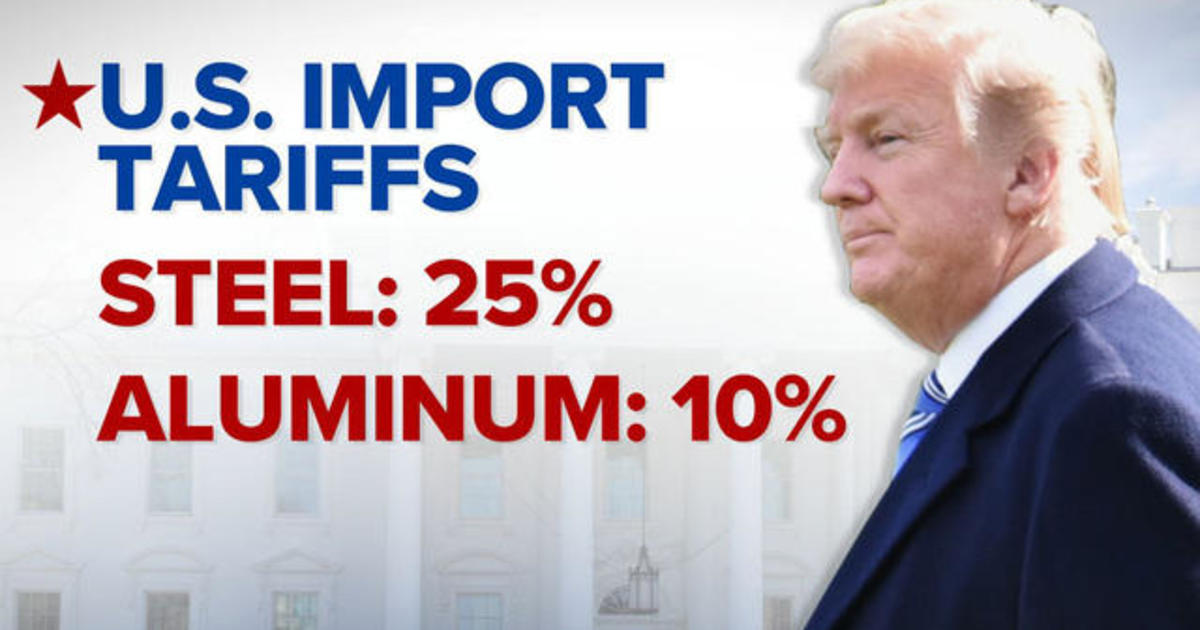
\includegraphics[width=\textwidth,height=4.6875in]{figures/trump_steel_tariff.jpeg}
\end{frame}

\begin{frame}{}
\protect\hypertarget{section-3}{}
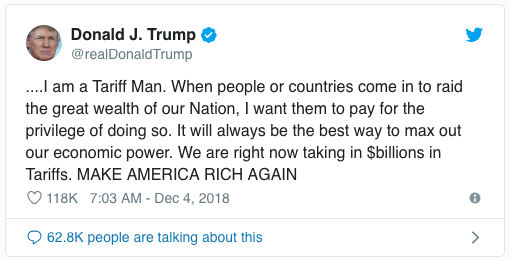
\includegraphics[width=\textwidth,height=4.6875in]{figures/tariff_man.png}
\end{frame}

\begin{frame}{}
\protect\hypertarget{section-4}{}
\includegraphics[width=\textwidth,height=4.6875in]{figures/trump_tariffs_tweet.jpeg}
\end{frame}

\begin{frame}{}
\protect\hypertarget{section-5}{}
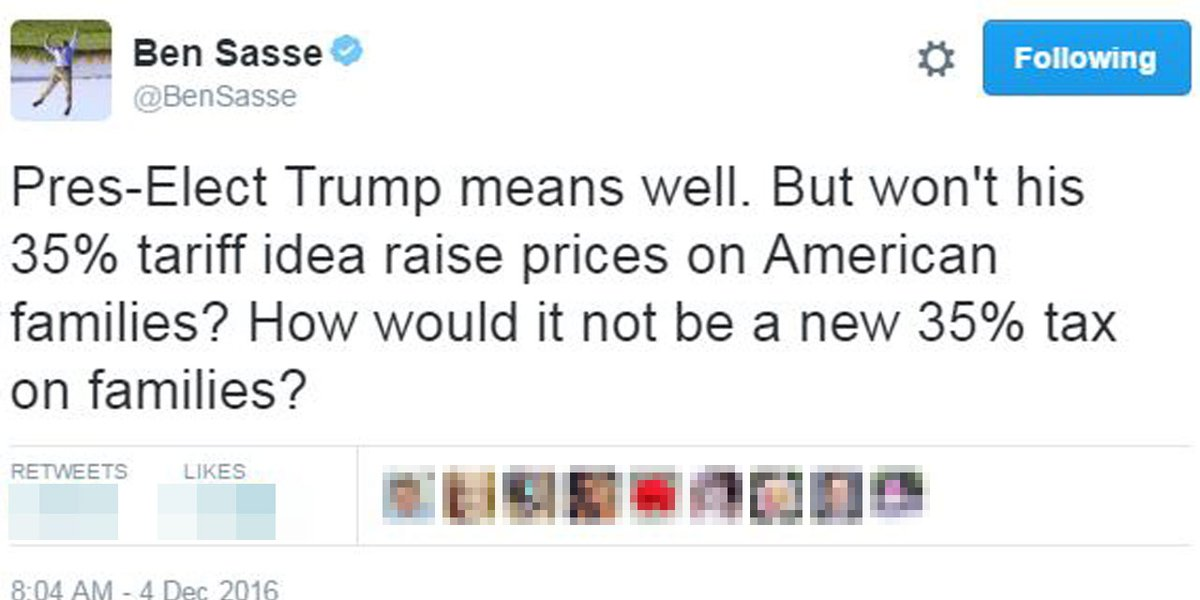
\includegraphics[width=\textwidth,height=4.6875in]{figures/sasse_tweet.jpeg}
\end{frame}

\begin{frame}{A simple model on tax}
\protect\hypertarget{a-simple-model-on-tax}{}
Say the government imposes a tax of \$40 on each night of hotel room
stay.

\begin{itemize}
\tightlist
\item
  How does that affect consumption?

  \begin{itemize}
  \tightlist
  \item
    Distortion; tax neutrality
  \end{itemize}
\item
  Who is paying for the tax?

  \begin{itemize}
  \tightlist
  \item
    Tax incidence
  \end{itemize}
\item
  What are the ``spillover'' effects?

  \begin{itemize}
  \tightlist
  \item
    Avoidance; evasion
  \end{itemize}
\end{itemize}
\end{frame}

\begin{frame}{}
\protect\hypertarget{section-6}{}
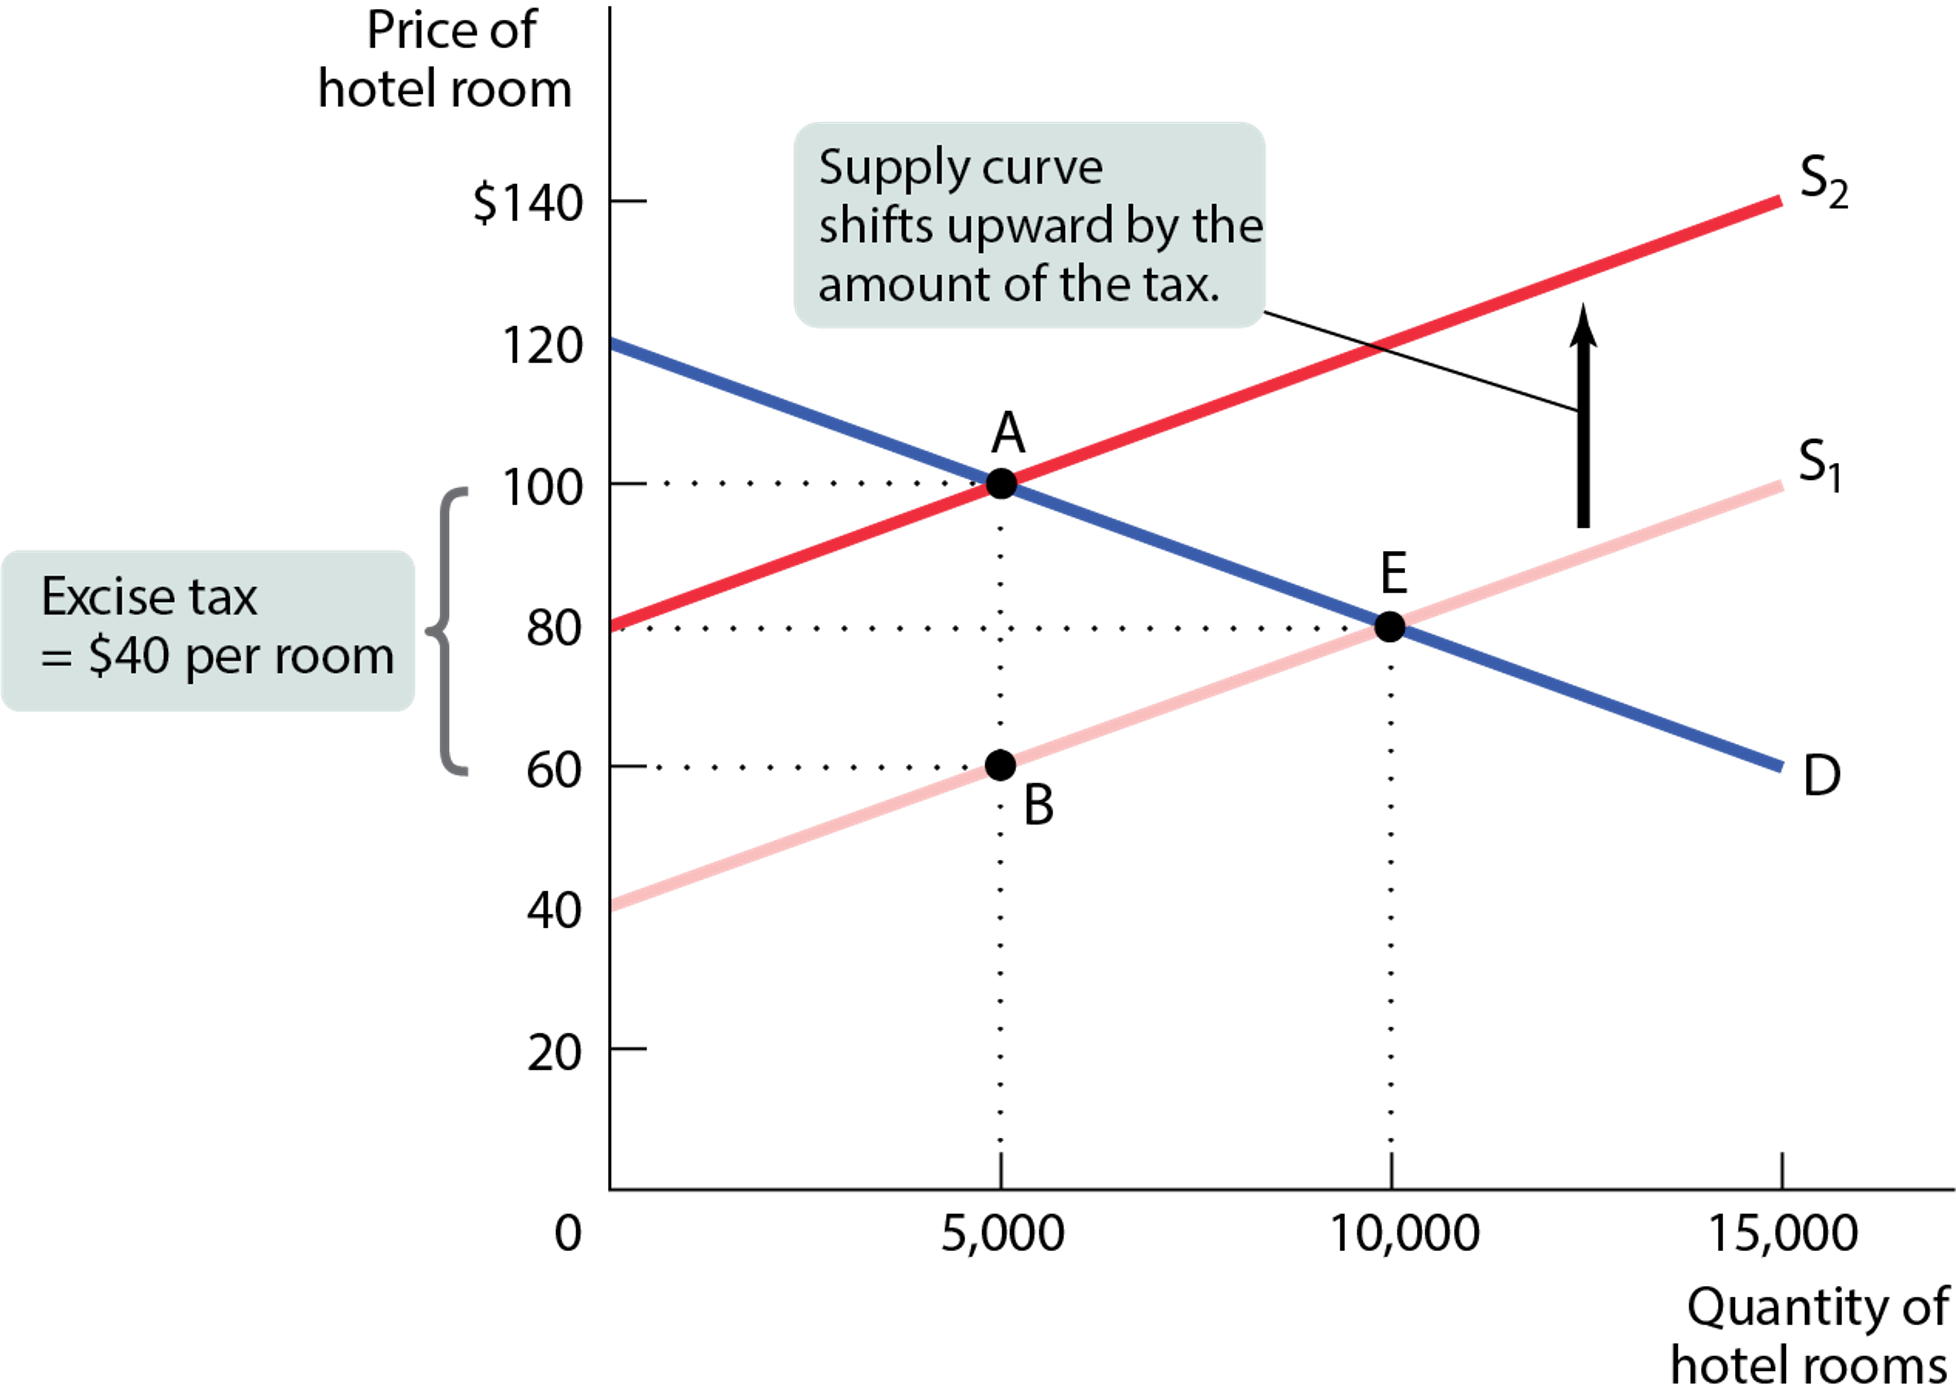
\includegraphics[width=\textwidth,height=4.6875in]{figures/fig14_2.png}
\end{frame}

\begin{frame}{}
\protect\hypertarget{section-7}{}
\begin{itemize}
\tightlist
\item
  The \$40 excise tax is shared between buyers and sellers.
\item
  The equilibrium price of hotel rooms falls to \$60 a night.
\item
  Hotel guests bear some of the burden as price paid by the guests
  (price plus tax) RISES from \$80 to \$100.
\item
  Hotel owners also bear some of the burden as their price FALLS from
  \$80 to \$60.
\end{itemize}
\end{frame}

\begin{frame}{}
\protect\hypertarget{section-8}{}
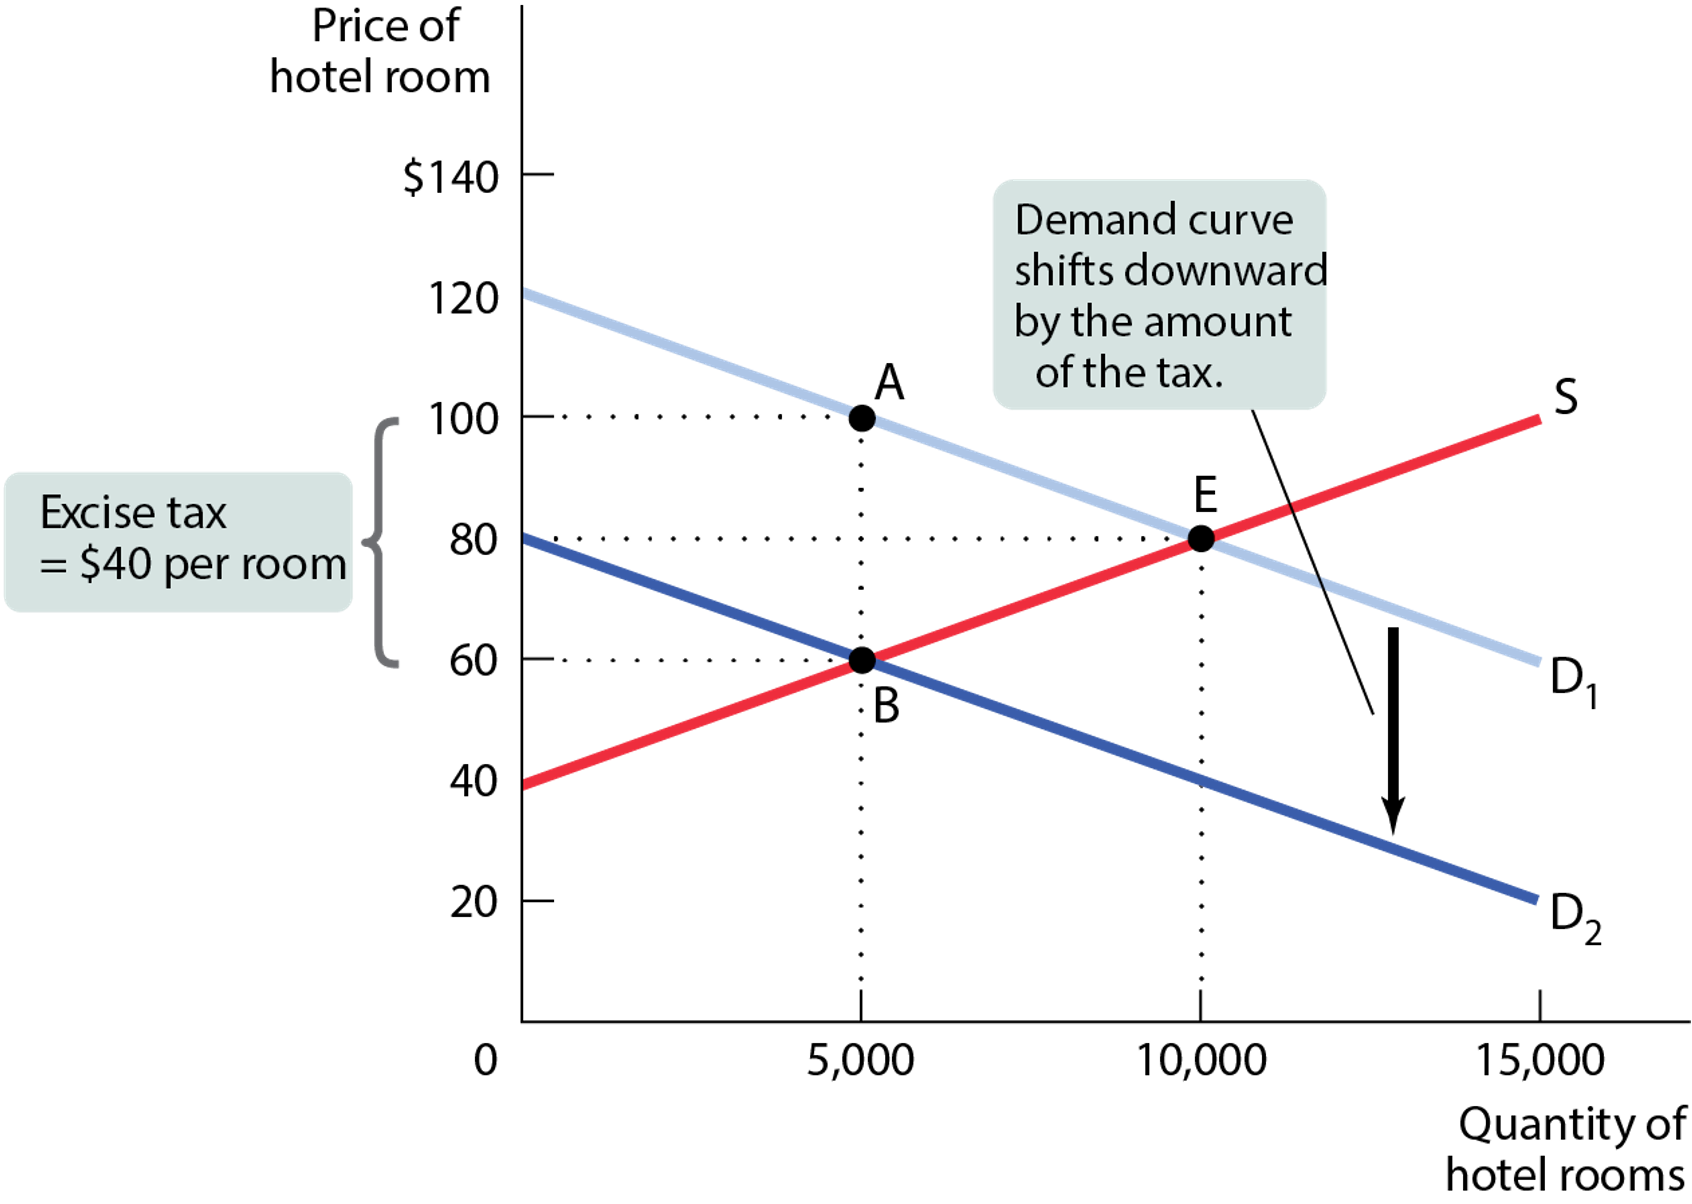
\includegraphics[width=\textwidth,height=4.6875in]{figures/fig14_3.png}
\end{frame}

\begin{frame}{}
\protect\hypertarget{section-9}{}
\begin{itemize}
\tightlist
\item
  It is not necessarily the case that consumers and producers bear equal
  burden of tax

  \begin{itemize}
  \tightlist
  \item
    In fact, it is rare that tax burden is equal
  \end{itemize}
\item
  In a long-distance relationship, for example, who will do more of the
  driving?
\end{itemize}
\end{frame}

\begin{frame}{}
\protect\hypertarget{section-10}{}
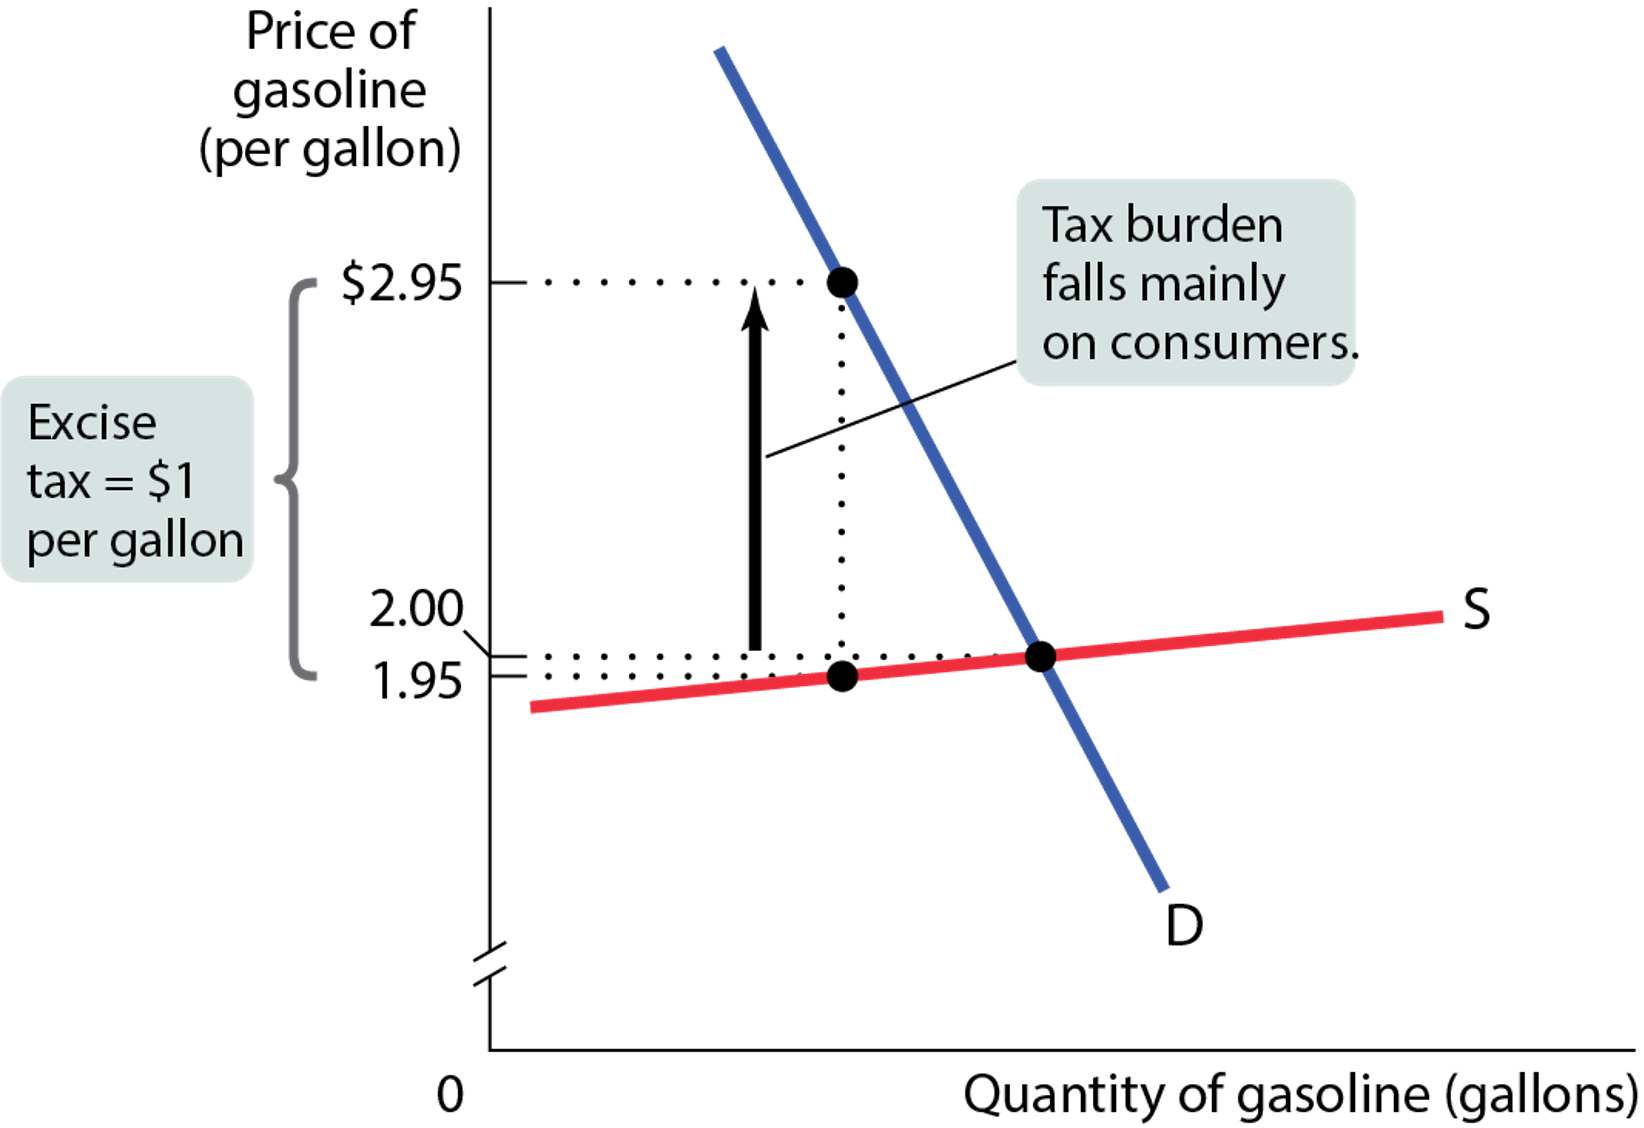
\includegraphics[width=\textwidth,height=4.6875in]{figures/fig14_4.png}
\end{frame}

\begin{frame}{}
\protect\hypertarget{section-11}{}
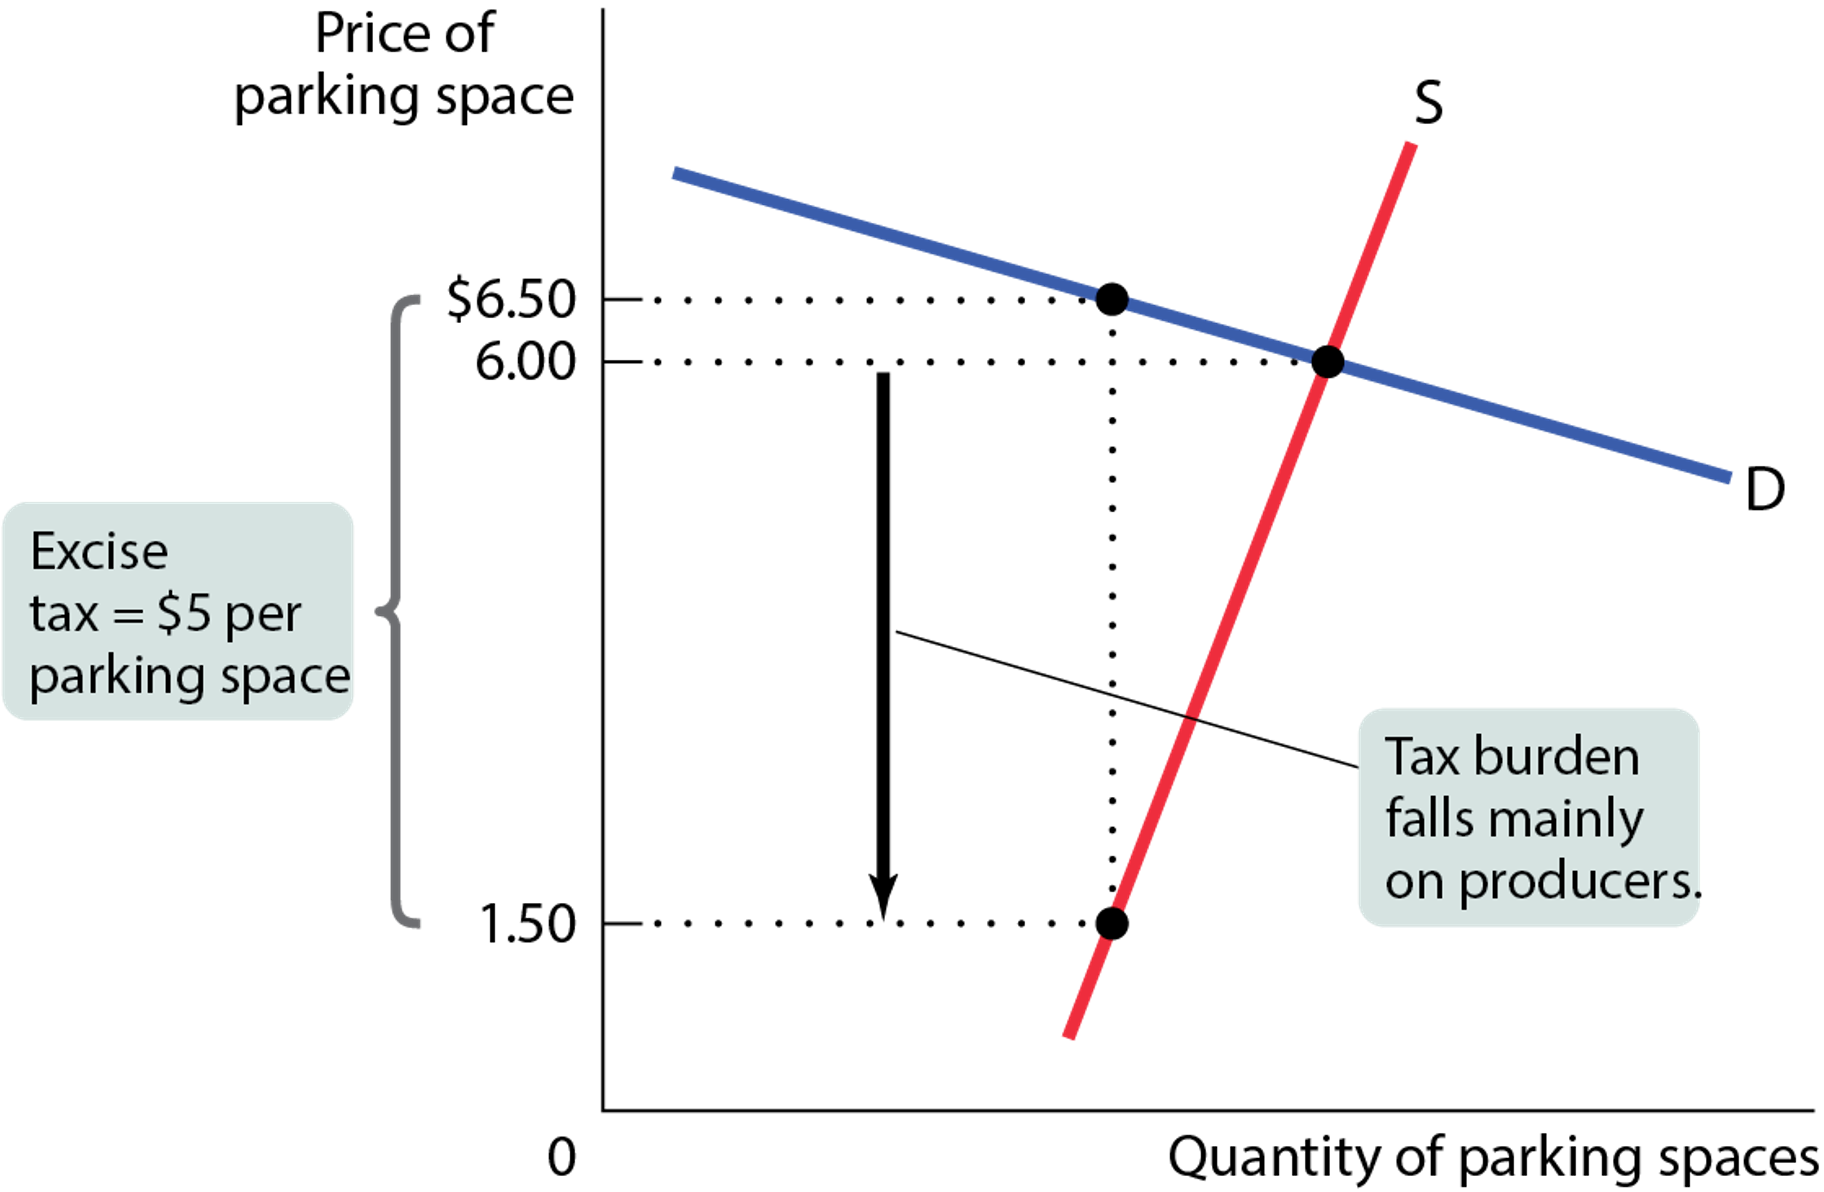
\includegraphics[width=\textwidth,height=4.6875in]{figures/fig14_5.png}
\end{frame}

\begin{frame}{}
\protect\hypertarget{section-12}{}
If demand of some good is more elastic than supply and a tax is imposed
on the consumption of the good, who will bear more of the burden of the
tax?

\begin{enumerate}
[a)]
\tightlist
\item
  producers, because consumers have a greater ability to change their
  behavior in response to the tax
\item
  both parties will share the burden equally
\item
  consumers, because they pay the tax out of pocket
\item
  the government, because the tax will cause less of the good to be
  produced and consumed
\end{enumerate}
\end{frame}

\begin{frame}{}
\protect\hypertarget{section-13}{}
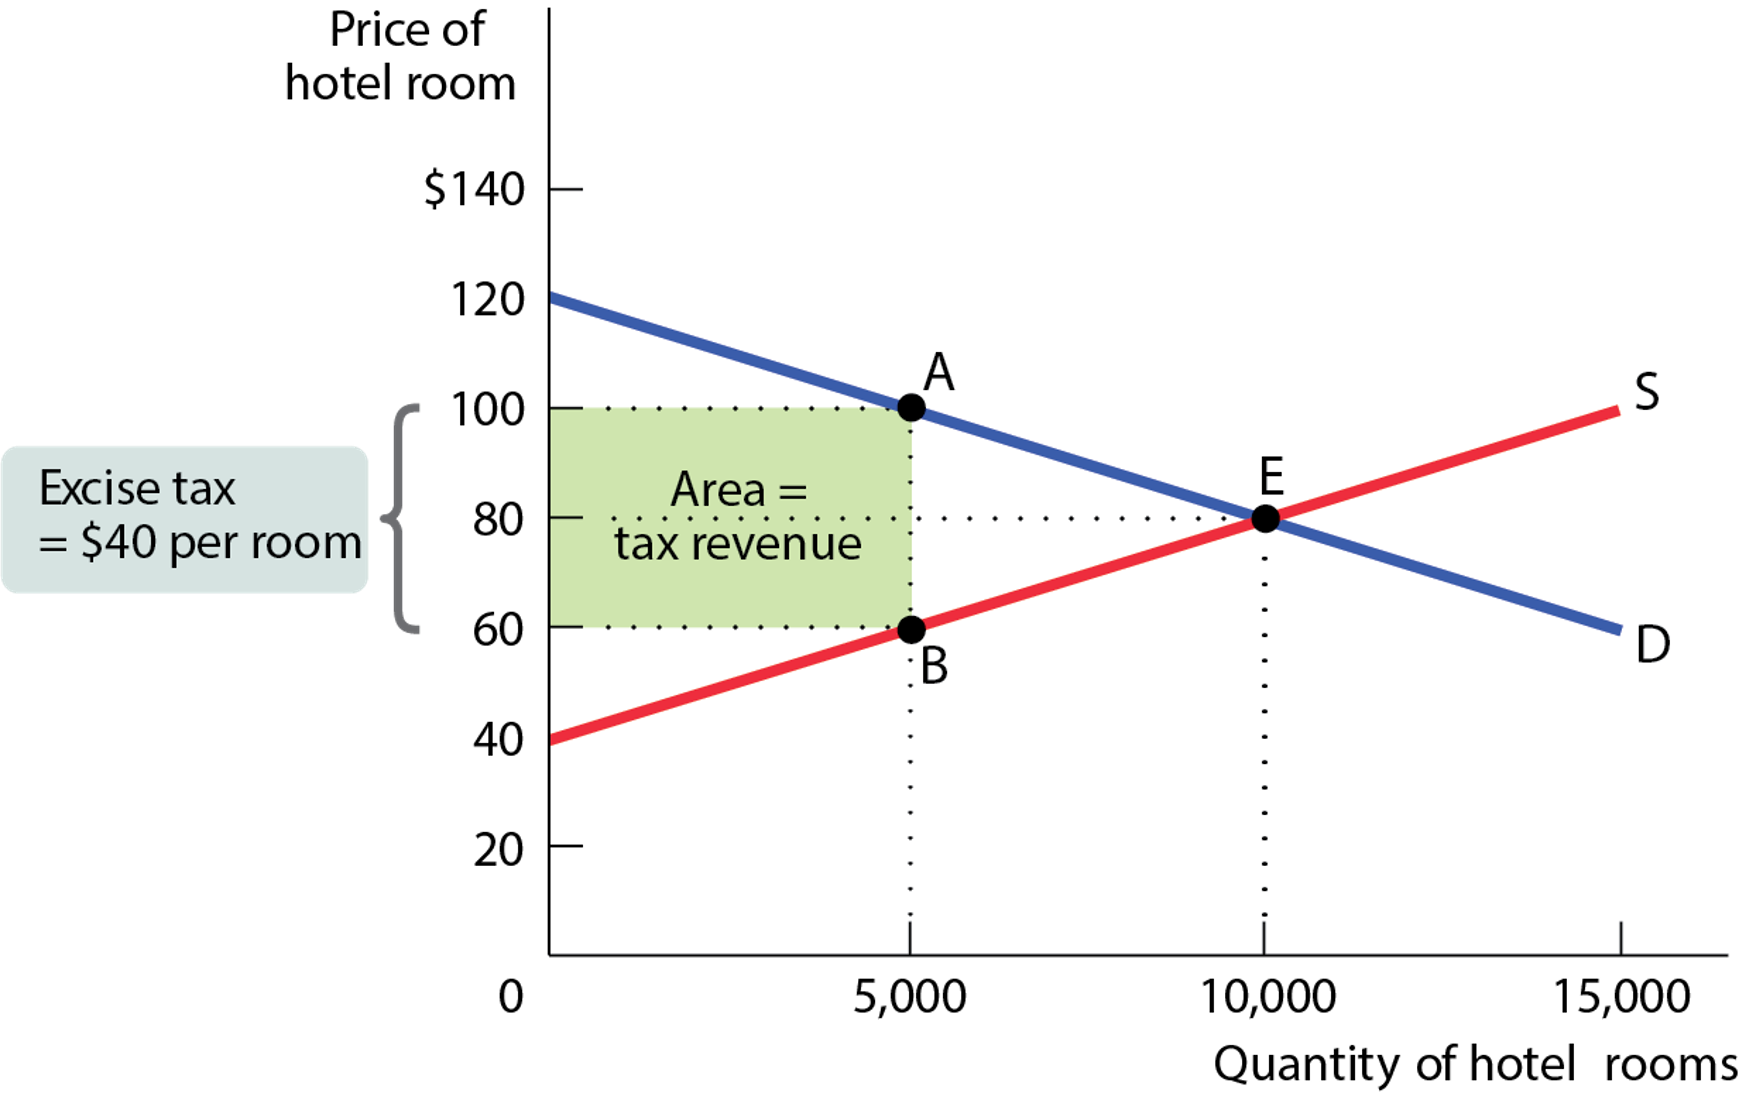
\includegraphics[width=\textwidth,height=4.6875in]{figures/fig14_6.png}
\end{frame}

\begin{frame}{}
\protect\hypertarget{section-14}{}
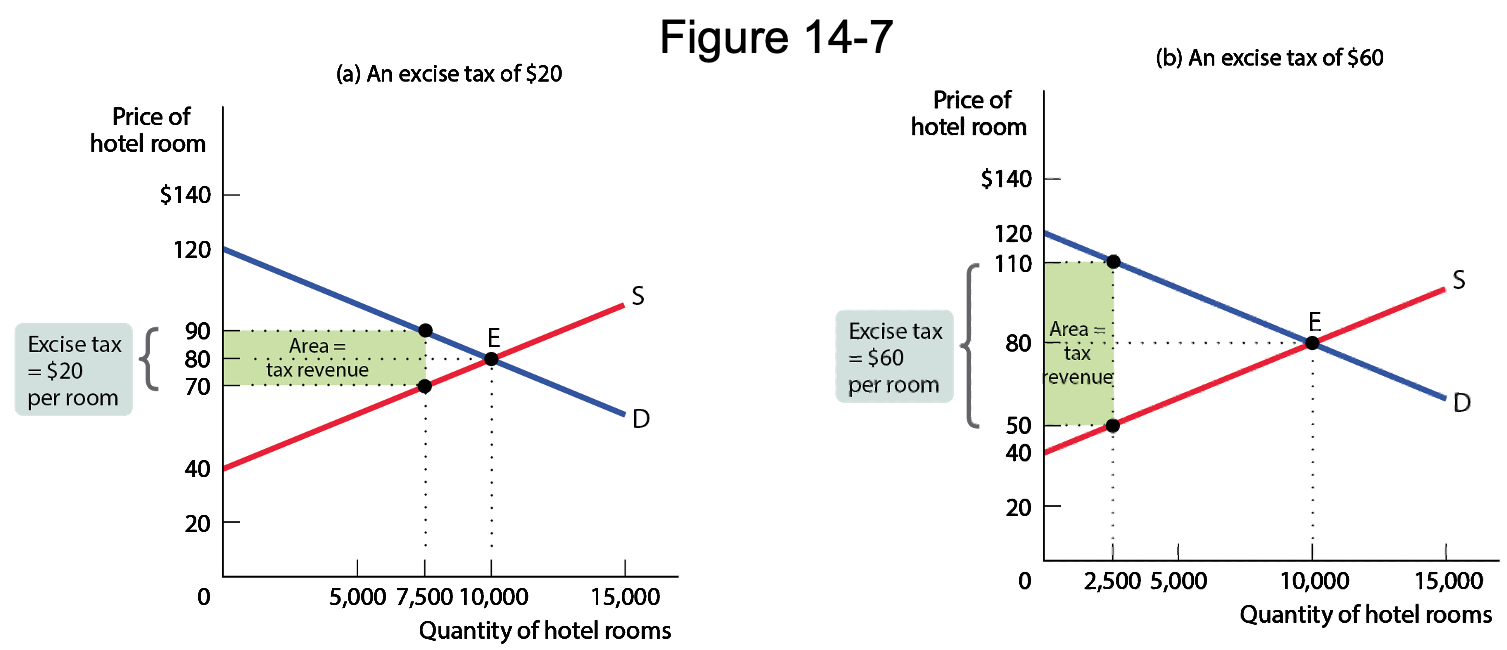
\includegraphics[width=\textwidth,height=4.6875in]{figures/fig14_7.png}
\end{frame}

\begin{frame}{Exercise tax creates distortion}
\protect\hypertarget{exercise-tax-creates-distortion}{}
\begin{itemize}
\tightlist
\item
  Deadweight loss is higher when

  \begin{itemize}
  \tightlist
  \item
    Demand is more elastic
  \item
    Supply is more elastic
  \end{itemize}
\item
  Deadweight loss is lower when

  \begin{itemize}
  \tightlist
  \item
    Both supply and demand are inelastic
  \end{itemize}
\end{itemize}
\end{frame}

\begin{frame}{}
\protect\hypertarget{section-15}{}
If we have to tax consumption, which of the followings should we tax in
order to minimize distortion?

\begin{itemize}
\tightlist
\item
  Gasoline
\item
  Apple
\item
  Apple Computer
\item
  Cigarette
\item
  Salt
\end{itemize}
\end{frame}

\begin{frame}{}
\protect\hypertarget{section-16}{}
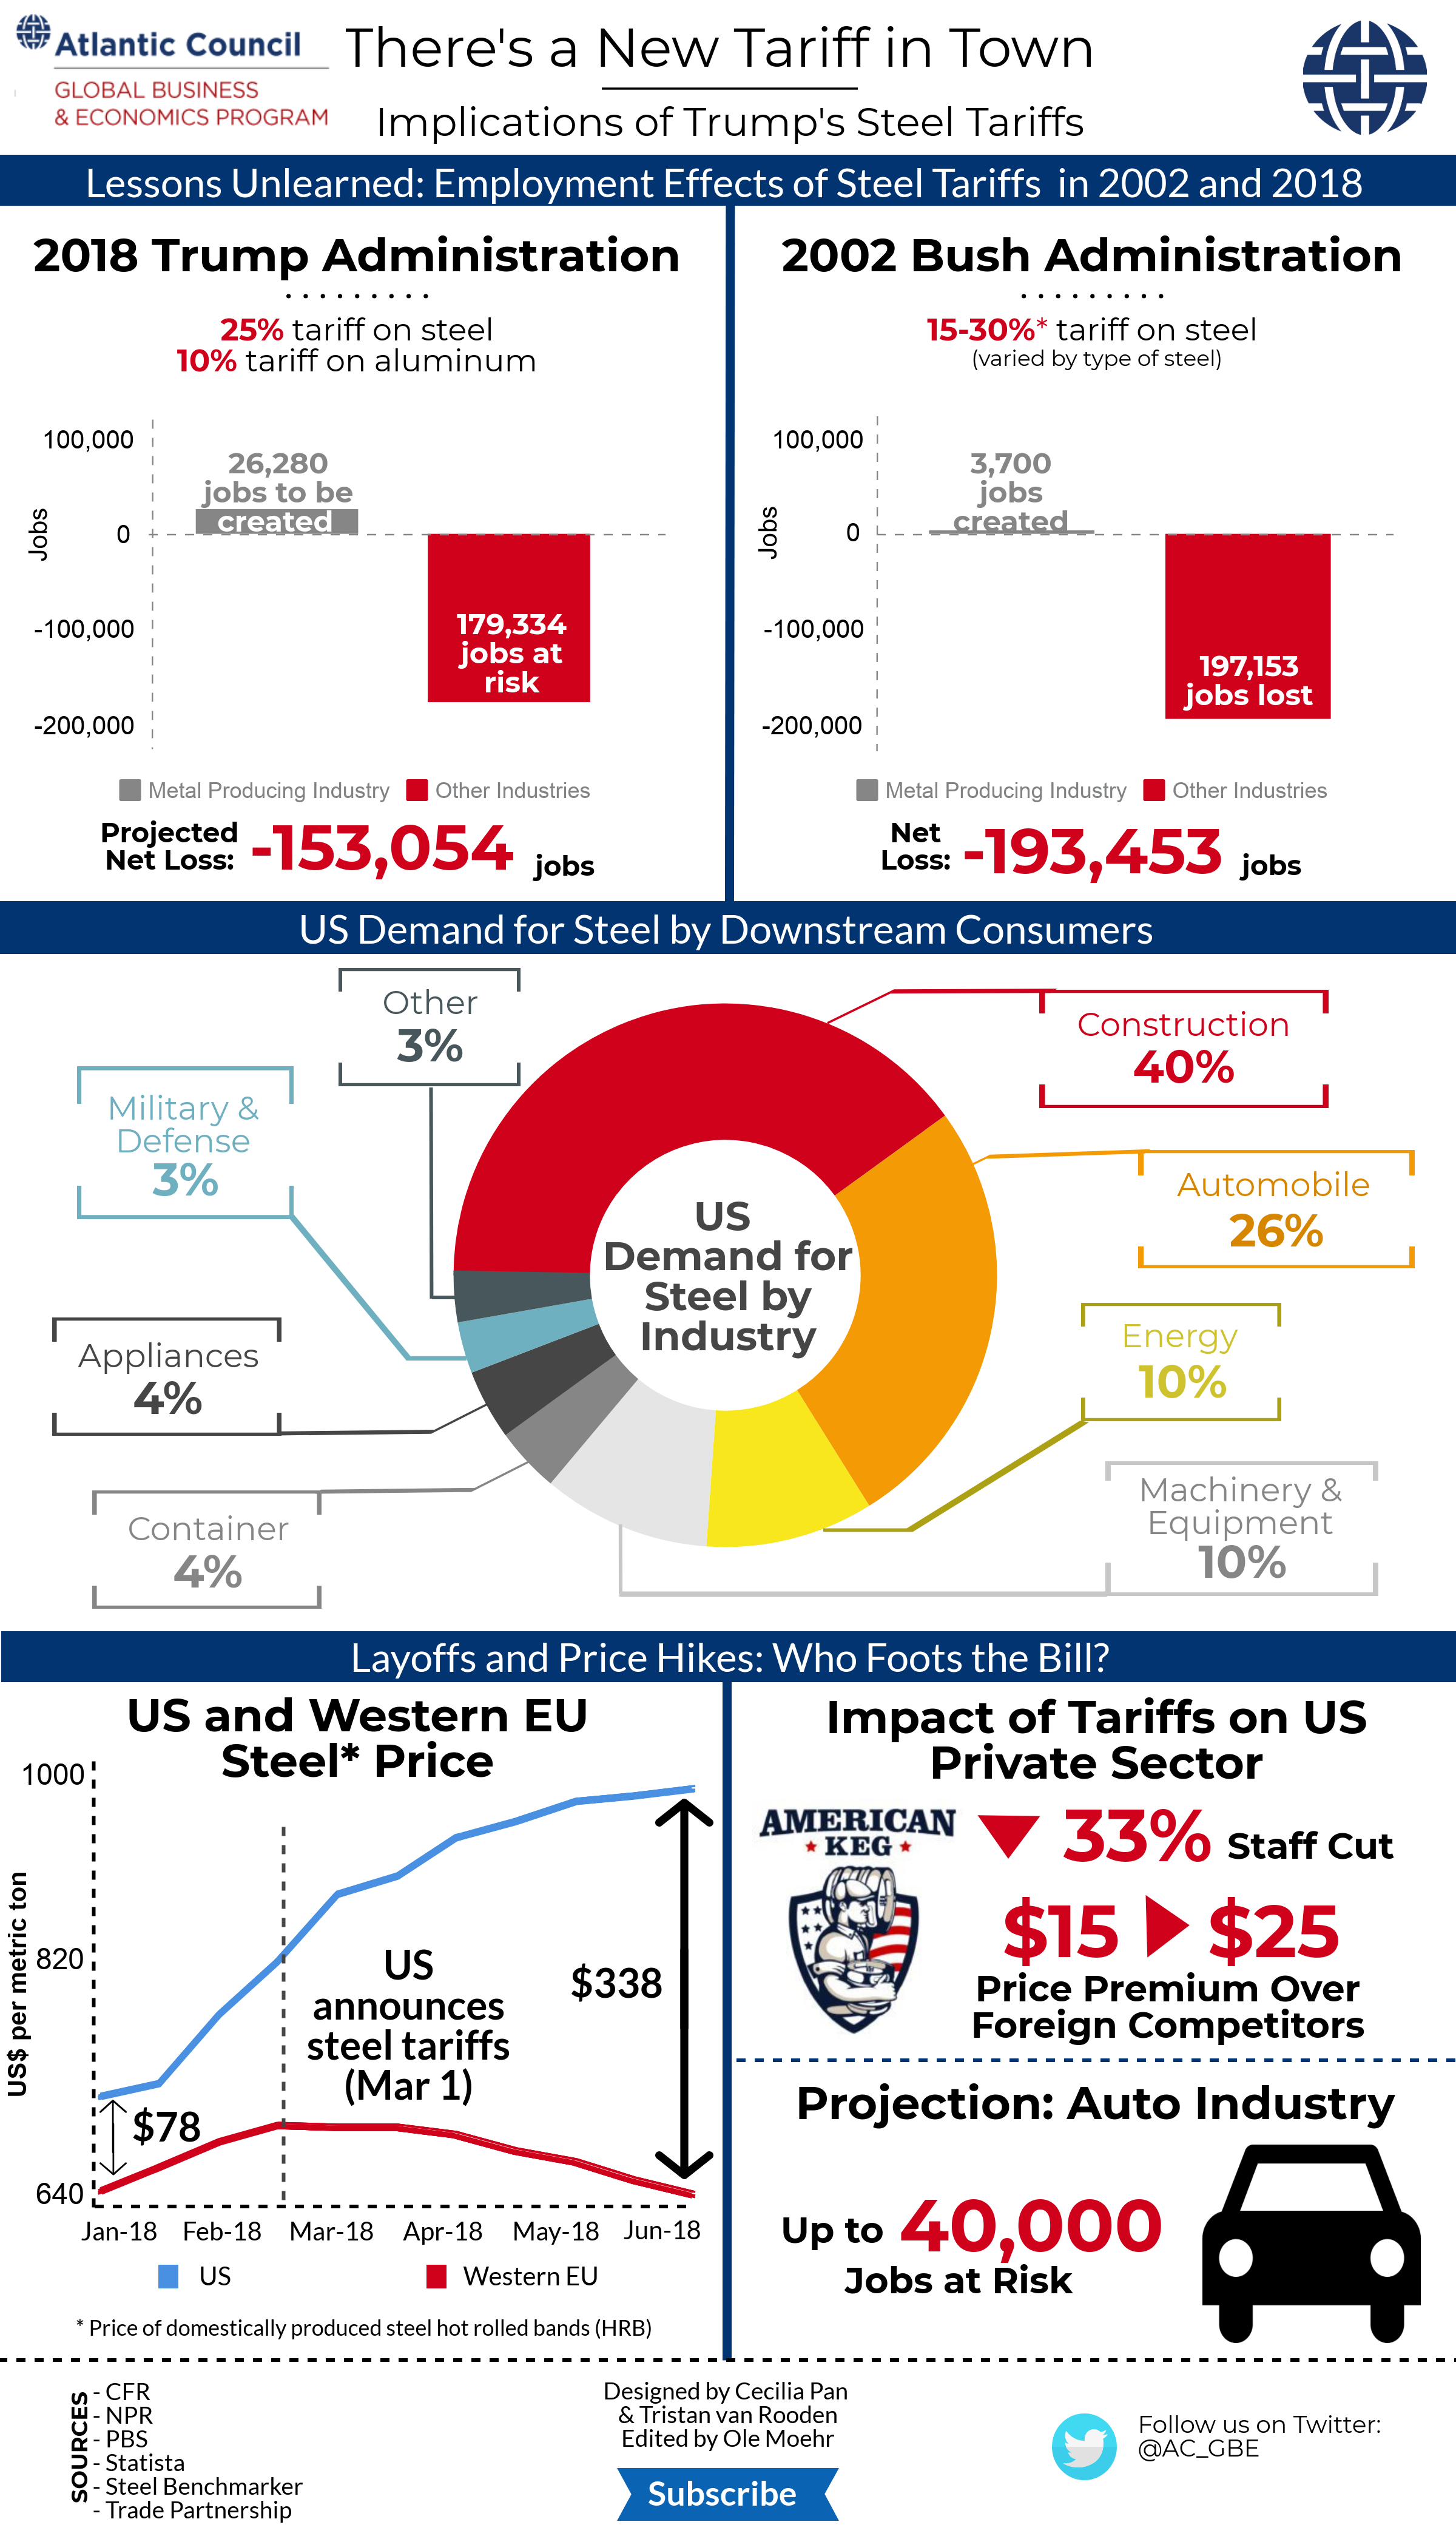
\includegraphics[width=\textwidth,height=7.8125in]{figures/steel_eg.png}
\end{frame}

\begin{frame}{}
\protect\hypertarget{section-17}{}
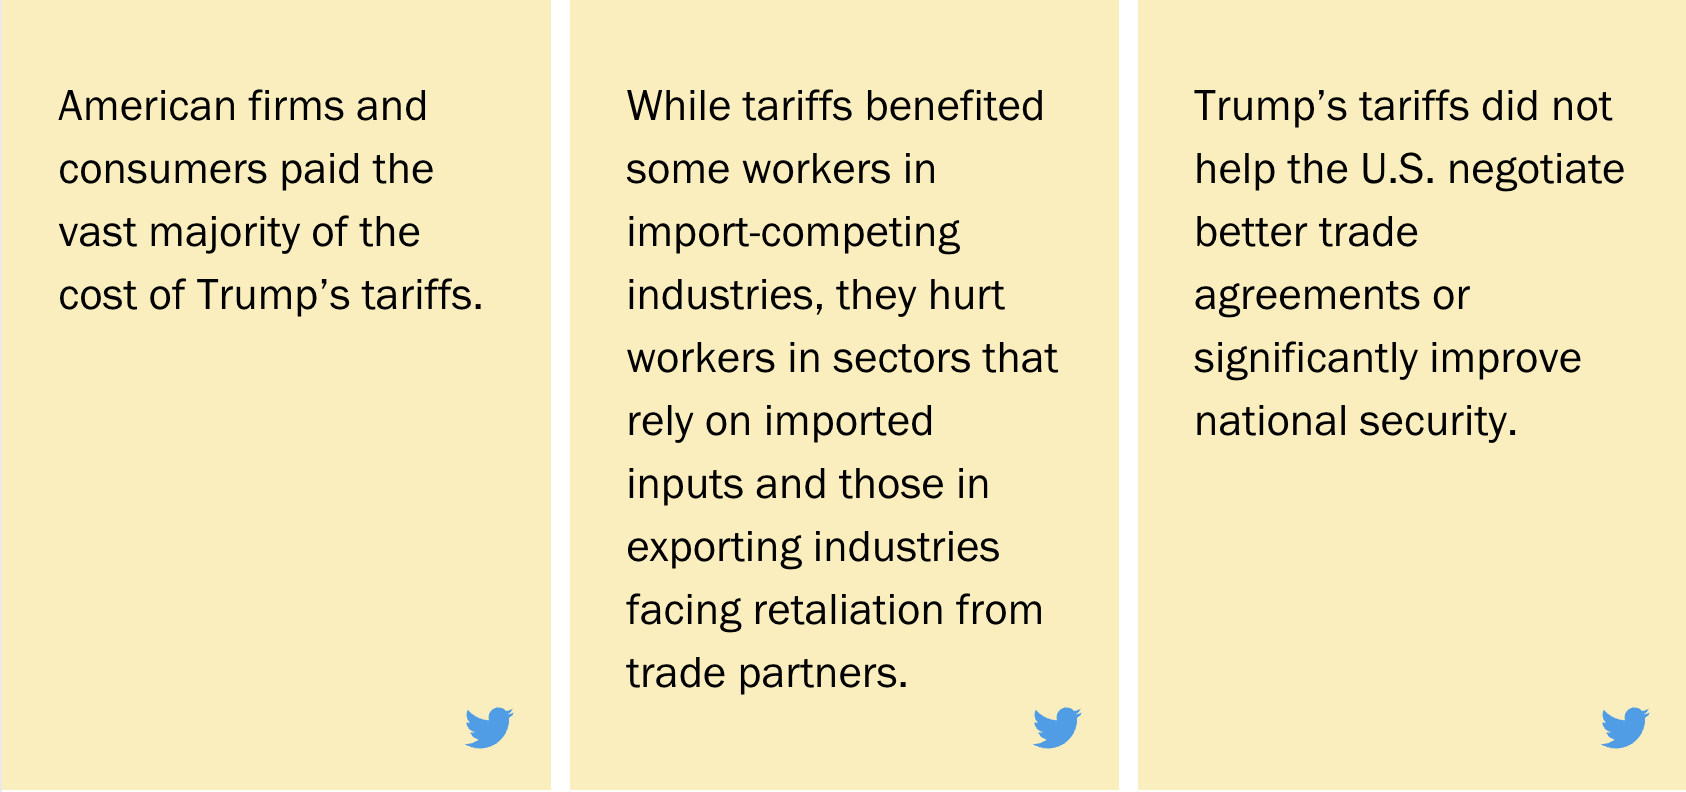
\includegraphics[width=\textwidth,height=7.8125in]{figures/brookings_tariff.png}
\end{frame}

\begin{frame}{Two remaining questions}
\protect\hypertarget{two-remaining-questions}{}
\begin{enumerate}
\tightlist
\item
  If tax is unavoidable
\end{enumerate}
\end{frame}

\begin{frame}{Back up a second}
\protect\hypertarget{back-up-a-second}{}
\begin{itemize}
\tightlist
\item
  Tax on regular items is ``bad'' because it creates distortion

  \begin{itemize}
  \tightlist
  \item
    If you tax one item, people 1) consumes less of it; 2) move to its
    substitutes
  \end{itemize}
\item
  Tax neutrality: economic decisions should be made based on economic
  merits, not tax reasons
\item
  Basic principle of taxation: lower tax rates and broaden tax base

  \begin{itemize}
  \tightlist
  \item
    If you tax everything at the same rate, there is no substitution
    effects
  \end{itemize}
\end{itemize}
\end{frame}

\begin{frame}{}
\protect\hypertarget{section-18}{}
In some instances, we may want tax to achieve specific goals - in those
cases tax is designed to be non-neutral: * Encourage home ownership *
Encourage health insurance adoption * Discourage carbon emission *
Discourage cigarette consumption
\end{frame}

\begin{frame}{}
\protect\hypertarget{section-19}{}
\end{frame}

\end{document}
